% =============================================================================
% CONFROUTE: Confidence-Aware Routing for Resilient Maritime Edge AI
% Talk for ICMIC 2026, NTUST Taipei, 19-21 August 2026.
% Oral slot: 15 min presentation + 2 min Q&A.
%
% Build:  latexmk -pdf slides.tex     (figures come from make_figures.py)
% =============================================================================
% NOTE: do not add xcolor=table here. colortbl breaks p{} columns in this
% MiKTeX/beamer build; our rows are highlighted with \hl instead of \rowcolor.
\documentclass[aspectratio=169, 11pt]{beamer}

\usepackage[T1]{fontenc}
\usepackage[utf8]{inputenc}
\usepackage[scaled=0.92]{helvet}
\renewcommand{\familydefault}{\sfdefault}
\usepackage{amsmath, amssymb}
\usepackage{array}      % required by colortbl for p{} columns
\usepackage{booktabs}
\usepackage{graphicx}
\usepackage{xcolor}
\usepackage{tikz}

\usetheme{default}
\usefonttheme{professionalfonts}
\setbeamertemplate{navigation symbols}{}
\setbeamertemplate{itemize items}[circle]

% --- palette (matches the generated figures) ---------------------------------
\definecolor{navy}{HTML}{104680}
\definecolor{cblue}{HTML}{2A78D6}
\definecolor{corange}{HTML}{EB6834}
\definecolor{caqua}{HTML}{1BAF7A}
\definecolor{ink}{HTML}{0B0B0B}
\definecolor{ink2}{HTML}{52514E}
\definecolor{muted}{HTML}{898781}
\definecolor{rule}{HTML}{E1E0D9}
\definecolor{wash}{HTML}{F4F7FB}
\definecolor{washorange}{HTML}{FDF0EA}

\setbeamercolor{normal text}{fg=ink}
\setbeamercolor{structure}{fg=navy}
\setbeamercolor{frametitle}{fg=navy}
\setbeamercolor{itemize item}{fg=cblue}
\setbeamercolor{itemize subitem}{fg=muted}
\setbeamerfont{frametitle}{size=\large, series=\bfseries}
\setbeamerfont{framesubtitle}{size=\small, series=\mdseries}
\setbeamercolor{framesubtitle}{fg=ink2}

\makeatletter
% frame title: bold navy line over a hairline rule
\setbeamertemplate{frametitle}{%
  \vspace{0.9em}%
  \begin{minipage}{\dimexpr\paperwidth-2\beamer@leftmargin\relax}%
    \raggedright\usebeamerfont{frametitle}\usebeamercolor[fg]{frametitle}%
    \insertframetitle\par
    \ifx\insertframesubtitle\@empty\else
      \vspace{0.15em}{\usebeamerfont{framesubtitle}\usebeamercolor[fg]{framesubtitle}\insertframesubtitle\par}%
    \fi
    \vspace{0.35em}{\color{rule}\hrule height 0.7pt}%
  \end{minipage}%
}

% footline: short title, venue, slide number
\setbeamertemplate{footline}{%
  \hbox{\begin{beamercolorbox}[wd=\paperwidth, ht=2.6ex, dp=1.4ex, leftskip=\beamer@leftmargin, rightskip=\beamer@rightmargin]{}%
    {\color{muted}\scriptsize CONFROUTE \quad\textbar\quad ICMIC 2026, NTUST Taipei}%
    \hfill{\color{muted}\scriptsize\insertframenumber}%
  \end{beamercolorbox}}%
}
\makeatother

% --- helpers -----------------------------------------------------------------
\newcommand{\shout}[1]{{\color{navy}\bfseries #1}}
\newcommand{\num}[1]{{\color{cblue}\bfseries #1}}
% highlights our own row in a results table
\newcommand{\hl}[1]{{\color{cblue}\bfseries #1}}

% a soft callout box
\newcommand{\callout}[2][wash]{%
  \begin{beamercolorbox}[wd=\textwidth, sep=0.55em]{}%
  \colorbox{#1}{\parbox{\dimexpr\textwidth-1.2em\relax}{\vspace{0.15em}#2\vspace{0.15em}}}%
  \end{beamercolorbox}}

% big centred statement frame
\newcommand{\statement}[2]{%
{\setbeamertemplate{footline}{}
\begin{frame}[plain]
  \vfill
  \begin{center}
    {\color{navy}\Large\bfseries #1}\\[0.8em]
    \begin{minipage}{0.78\textwidth}\centering\color{ink2}\normalsize #2\end{minipage}
  \end{center}
  \vfill
\end{frame}}}

\title{CONFROUTE}
\author{Anthony Uchenna Eneh}
\date{August 2026}

\begin{document}

% =============================================================================
% 1. Title
% =============================================================================
{\setbeamertemplate{footline}{}
\begin{frame}[plain]
  \vspace{0.9em}
  {\color{muted}\footnotesize The 5th International Conference on Mobile, Military and Maritime IT Convergence (ICMIC 2026)\\
   National Taiwan University of Science and Technology, Taipei \quad\textbar\quad 19--21 August 2026}

  \vspace{1.6em}
  {\color{navy}\huge\bfseries CONFROUTE}\\[0.35em]
  {\color{ink}\Large Confidence-Aware Routing for\\[0.15em] Resilient Maritime Edge AI}

  \vspace{1.3em}
  {\color{rule}\hrule height 0.7pt}
  \vspace{1.0em}

  {\normalsize \textbf{Anthony Uchenna Eneh}$^{1}$, \enspace Love Allen Chijioke Ahakonye$^{2}$,\\[0.2em]
   Jae Min Lee$^{1}$, \enspace Dong-Seong Kim$^{1,\ast}$}

  \vspace{0.7em}
  {\color{ink2}\footnotesize
   $^{1}$IT-Convergence Engineering, Kumoh National Institute of Technology, Gumi, South Korea\\
   $^{2}$ICT Convergence Research Center, Kumoh National Institute of Technology, Gumi, South Korea\\
   $^{\ast}$NSLab Co. Ltd., Gumi, South Korea}

  \vfill
  {\color{muted}\scriptsize anthony@kumoh.ac.kr}
  \vspace{0.4em}
\end{frame}}

% =============================================================================
% 2. Motivation
% =============================================================================
\begin{frame}{A vessel has to decide on its own}
\framesubtitle{Perception, monitoring, video triage and navigation support now run at the maritime edge}

\vspace{0.3em}
\begin{columns}[T]
\begin{column}{0.52\textwidth}
  \textbf{\color{navy}What the platform is up against}
  \begin{itemize}\setlength\itemsep{0.55em}
    \item \textbf{Links come and go.} Satellite and ship-to-ship connectivity is intermittent by nature.
    \item \textbf{Compute is small.} Onboard power and thermal budgets are fixed.
    \item \textbf{The sea changes the input.} Sea state, illumination, haze and occlusion shift the data away from training.
    \item \textbf{Errors outrank latency.} A wrong safety-critical decision costs far more than a slow one.
  \end{itemize}
\end{column}
\begin{column}{0.45\textwidth}
  \vspace{1.6em}
  \callout{\small The question this paper asks:\\[0.5em]
  {\color{navy}\bfseries When should an edge node act on its own model, hand the task off, or refuse to decide?}}

  \vspace{0.8em}
  {\color{ink2}\small Cloud-centric pipelines answer only the first two.}
\end{column}
\end{columns}
\end{frame}

% =============================================================================
% 3. The gap
% =============================================================================
\begin{frame}{What existing maritime offloading assumes}
\framesubtitle{Bandit scheduling, distributed optimisation and multi-agent RL all optimise latency against energy}

\vspace{0.6em}
\begin{columns}[T]
\begin{column}{0.47\textwidth}
  \callout[wash]{\textbf{\color{navy}Assumption 1}\\[0.4em]
  The remote node is \emph{reachable}, so offloading is always an available escape hatch.}
  \vspace{0.9em}
  \callout[wash]{\textbf{\color{navy}Assumption 2}\\[0.4em]
  The model's confidence is \emph{trustworthy}, so a threshold on it is a safe gate.}
\end{column}
\begin{column}{0.50\textwidth}
  \textbf{\color{corange}Both fail at sea.}
  \begin{itemize}\setlength\itemsep{0.5em}
    \item Under degraded links there is often \emph{no} peer to offload to.
    \item Under maritime image degradation, confidence does not track correctness. We measured this, and it is worse than ``uninformative''.
  \end{itemize}
  \vspace{0.6em}
  {\color{ink2}\small Uncertainty-aware edge scheduling exists, but treats uncertainty as an input to allocation, never as a trigger to \emph{stop}.}
\end{column}
\end{columns}
\end{frame}

% =============================================================================
% 4. The hook: calibration failure
% =============================================================================
\begin{frame}{Measurement first: is confidence trustworthy under sea conditions?}
\framesubtitle{ResNet-18 vessel classifier, 500 held-out ShipsNet chips, deterministic adverse transform}

\vspace{-0.2em}
\begin{columns}[c]
\begin{column}{0.62\textwidth}
  \centering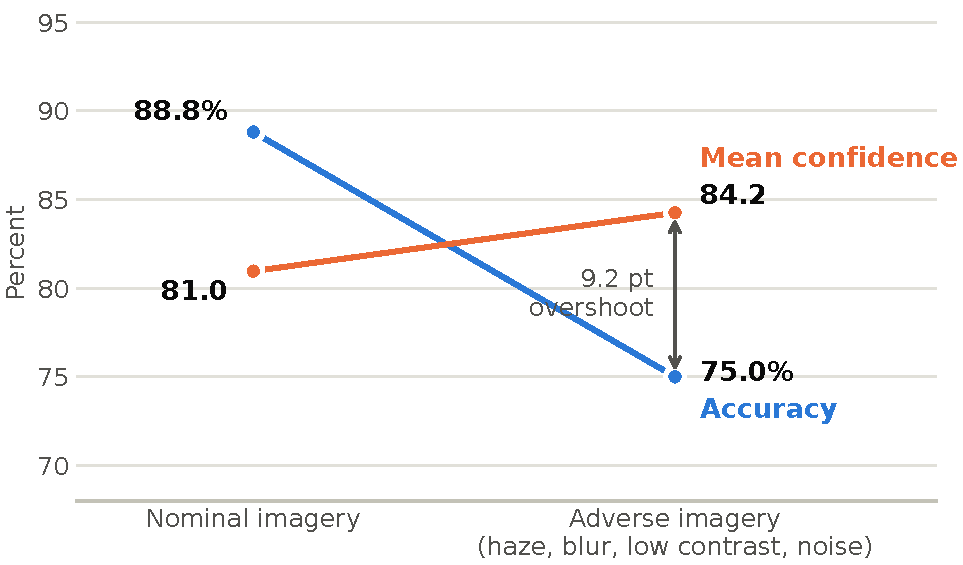
\includegraphics[width=\linewidth]{figures/fig_calibration.pdf}
\end{column}
\begin{column}{0.36\textwidth}
  \callout[washorange]{\small Accuracy falls to \num{75.0\%},\\ yet mean confidence \emph{rises} to \num{0.842}.}

  \vspace{0.7em}
  {\small The model does not merely lose information under degradation. It becomes \shout{more certain while being more wrong}.}

  \vspace{0.7em}
  {\color{ink2}\small Mean confidence on \emph{incorrect} predictions climbs from 0.651 to 0.782.}
\end{column}
\end{columns}
\end{frame}

% =============================================================================
% 5. Consequence for threshold offloading
% =============================================================================
\begin{frame}{So a confidence threshold cannot see the errors that matter}
\framesubtitle{Where the classifier's mistakes actually sit, relative to a 0.65 fallback threshold}

\vspace{-0.3em}
\centering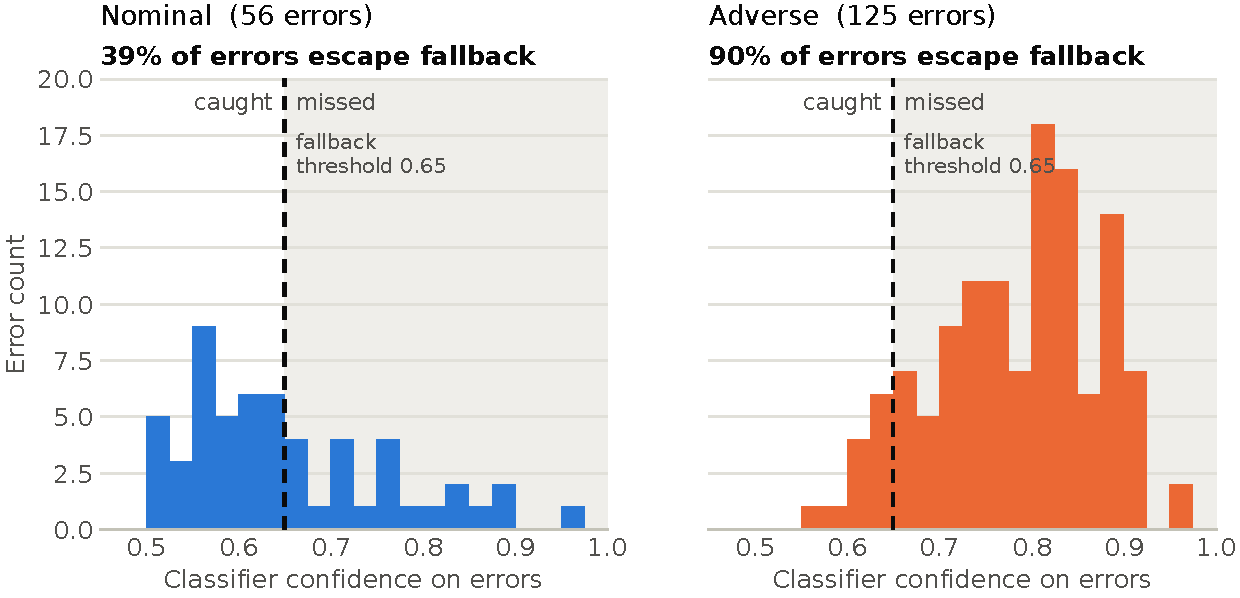
\includegraphics[width=0.80\textwidth]{figures/fig_error_confidence.pdf}

\vspace{0.2em}
\begin{minipage}{0.86\textwidth}
\callout[washorange]{\small Exactly when conditions get hard, the errors a confidence gate would miss go from \num{39\%} to \num{90\%}.}
\end{minipage}
\end{frame}

% =============================================================================
% 6. Contributions
% =============================================================================
\begin{frame}{What we contribute}

\vspace{0.8em}
\begin{enumerate}\setlength\itemsep{1.0em}
  \item[\textbf{\color{cblue}1}] \textbf{A three-way routing policy} over \emph{local}, \emph{forward} and \emph{fallback}, driven by confidence, queue load, urgency and link quality. Fallback is a first-class action, not a post-failure mode.
  \item[\textbf{\color{cblue}2}] \textbf{An evaluation over 37,500 routing decisions} on real ShipsNet imagery and three maritime link regimes, showing that under degraded connectivity CONFROUTE cuts unsafe outcomes from 6.8\% to 4.8\% against always-offload, while being 40 ms faster.
  \item[\textbf{\color{cblue}3}] \textbf{A negative result we think matters more:} unsafe outcomes persist \emph{despite} high confidence. Calibration, not routing policy design, is the binding constraint on maritime edge AI reliability.
\end{enumerate}
\end{frame}

% =============================================================================
% 7. Architecture
% =============================================================================
\begin{frame}{CONFROUTE sits after inference and before actuation}
\framesubtitle{The router consumes uncertainty without touching the model, and logs every decision for audit}

\vspace{-0.3em}
\centering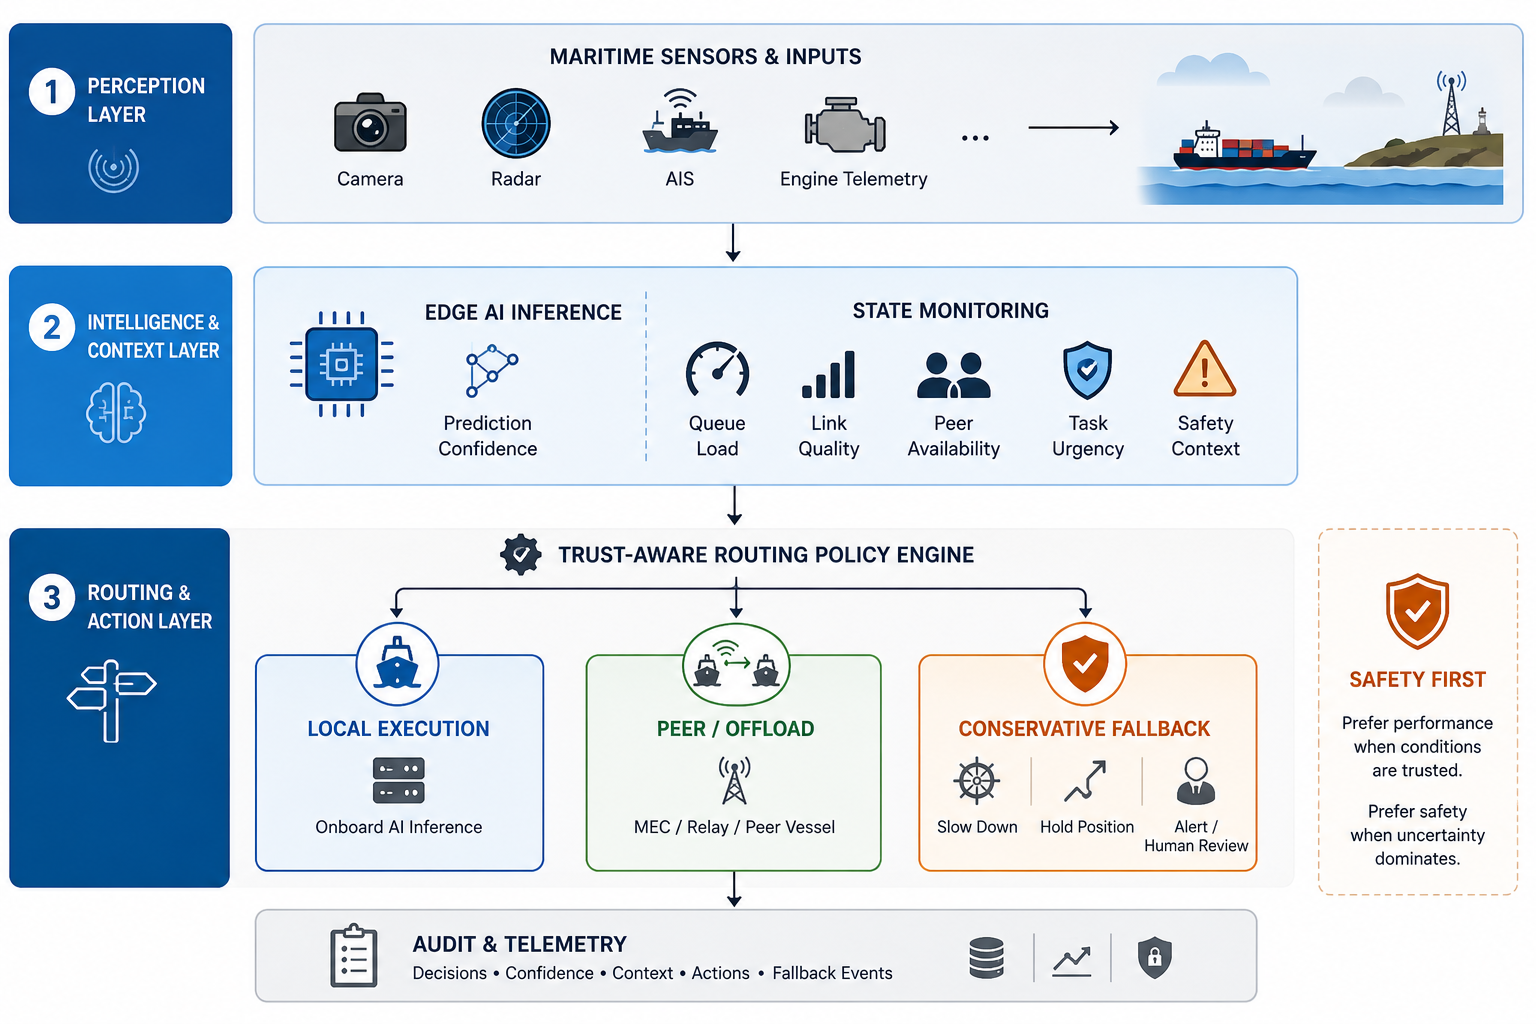
\includegraphics[height=0.70\textheight]{../paper/figures/architecture_full.png}
\end{frame}

% =============================================================================
% 8. Fallback is the point
% =============================================================================
\begin{frame}{``Fallback'' is an operational action, not an error code}
\framesubtitle{What the conservative branch means, per maritime application}

\vspace{0.5em}
\centering
{\small\raggedright
\begin{tabular}{@{}>{\raggedright\arraybackslash}p{0.27\textwidth} >{\raggedright\arraybackslash}p{0.30\textwidth} >{\raggedright\arraybackslash}p{0.36\textwidth}@{}}
\toprule
\textbf{\color{navy}Application} & \textbf{\color{navy}Full inference} & \textbf{\color{navy}Fallback action} \\
\midrule
Collision avoidance & Predict intent of nearby vessel & Reduce speed, sound horn, hold heading, alert operator \\[0.45em]
Maritime surveillance & Classify ship / no-ship chip & Flag for review, defer alert, request another pass \\[0.45em]
Engine anomaly & Classify fault from vibration spectrogram & Report ``inspection needed'', use a limit-based alert \\[0.45em]
Waypoint decision & Select path from camera and LiDAR & Hold position, revert to last safe heading, request human review \\
\bottomrule
\end{tabular}}

\vspace{0.8em}
{\color{ink2}\small Each of these is auditable and aligned with COLREGS/IMO practice: the ship does something conservative and says why.}
\end{frame}

% =============================================================================
% 9. Policy
% =============================================================================
\begin{frame}{The policy: three scores, then guardrails}

\vspace{0.2em}
\begin{columns}[T]
\begin{column}{0.54\textwidth}
  {\color{ink2}\small Confidence $c_i$, uncertainty $z_i = 1-c_i$, normalised queue $\bar q_i$, link quality $\ell_i$, urgency $\kappa_i$, safety flag $\phi_i$.}
  \vspace{0.5em}
  \begin{align*}
    S_{\text{local}}    &= \alpha c_i - \beta \bar q_i + \gamma \kappa_i \\[0.25em]
    S_{\text{forward}}  &= \lambda \ell_i + \mu \bar q_i - \nu z_i \\[0.25em]
    S_{\text{fallback}} &= \rho z_i + \eta (1-\ell_i) + \delta \phi_i
  \end{align*}
  \vspace{0.1em}
  {\color{ink2}\small Pick the highest score, subject to hard guardrails.}
\end{column}
\begin{column}{0.43\textwidth}
  \callout[wash]{\textbf{\color{navy}Guardrails override the scores}
  \begin{itemize}\setlength\itemsep{0.35em}\small
    \item No forwarding when no peer is available or $\ell_i$ is below the link floor.
    \item No local execution on a safety-sensitive task below the confidence floor.
  \end{itemize}}
  \vspace{0.7em}
  {\small A \shout{threshold controller}, deliberately. It is inspectable, certifiable, and tunable from traces. A learned policy is none of those things on a bridge.}
\end{column}
\end{columns}
\end{frame}

% =============================================================================
% 10. Decision regions
% =============================================================================
\begin{frame}{The deployed decision regions}
\framesubtitle{Fallback requires both signals to fail: confidence below 0.65 \emph{and} bandwidth below 1.8 Mbps}

\vspace{-0.2em}
\begin{columns}[c]
\begin{column}{0.58\textwidth}
  \centering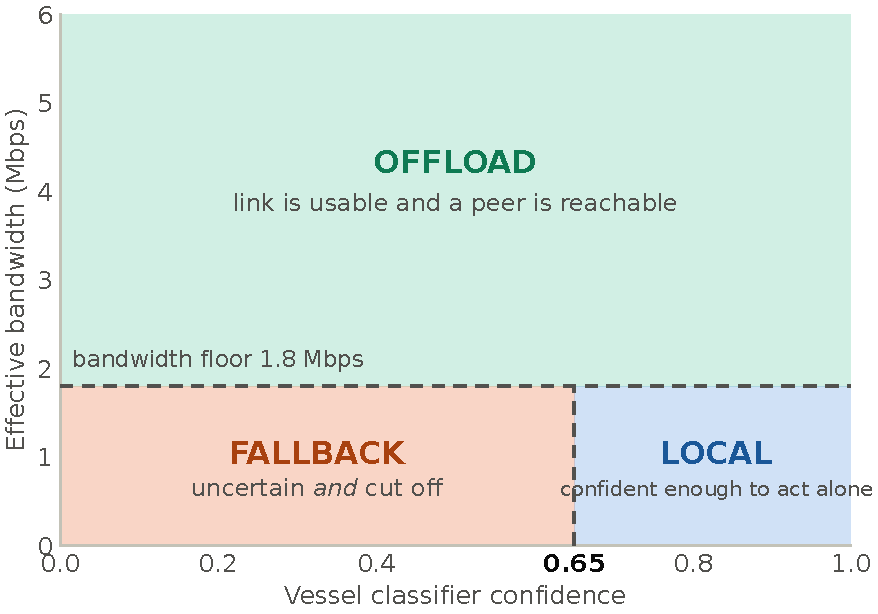
\includegraphics[width=\linewidth]{figures/fig_boundary.pdf}
\end{column}
\begin{column}{0.40\textwidth}
  {\small Requiring \emph{both} conditions keeps fallback rare and purposeful.}
  \vspace{0.8em}

  {\small The router never refuses to decide simply because the model is unsure, if the link is healthy enough to ask someone better.}
  \vspace{0.8em}

  {\color{ink2}\small Thresholds are calibrated offline from traces; queue and link estimates update online without retraining.}
\end{column}
\end{columns}
\end{frame}

% =============================================================================
% 11. Setup
% =============================================================================
\begin{frame}{Experimental setup}

\vspace{0.4em}
\begin{columns}[T]
\begin{column}{0.47\textwidth}
  \textbf{\color{navy}Classifier and traces}
  \begin{itemize}\setlength\itemsep{0.15em}\small
    \item ShipsNet: 4,000 PlanetScope $80\times80$ chips, 1,000 ship / 3,000 no-ship.
    \item ResNet-18, ImageNet-initialised, 2,800 / 600 / 600 split, 84.8\% validation accuracy.
    \item Confidence traces from 500 held-out chips, nominal and adverse.
  \end{itemize}
  \vspace{0.7em}
  \textbf{\color{navy}Workload}
  \begin{itemize}\setlength\itemsep{0.15em}\small
    \item 2,500 tasks per policy per regime: \shout{37,500 decisions}.
    \item Adverse traces with probability 0.4; 30\% safety-sensitive.
  \end{itemize}
\end{column}
\begin{column}{0.49\textwidth}
  \textbf{\color{navy}Three link regimes}

  \vspace{0.35em}
  {\footnotesize
  \begin{tabular}{@{}lrrrr@{}}
  \toprule
   & \textbf{Mbps} & \textbf{Avail.} & \textbf{Loss} & \textbf{Base} \\
  \midrule
  Stable       & 5--12    & 90\% & 3\%  & 20\,ms \\
  Intermittent & 0.8--6   & 70\% & 12\% & 40\,ms \\
  Degraded     & 0.2--2.5 & 40\% & 30\% & 80\,ms \\
  \bottomrule
  \end{tabular}}

  \vspace{0.9em}
  \textbf{\color{navy}Four baselines}
  \begin{itemize}\setlength\itemsep{0.2em}\small
    \item Always local
    \item Always offload (availability-aware)
    \item Confidence threshold ($<0.70$)
    \item Load only ($\bar q > 0.5$)
  \end{itemize}
\end{column}
\end{columns}

\vspace{0.3em}
{\color{ink2}\scriptsize \textbf{Unsafe rate} = routing-layer risk: safety-sensitive local errors, low-confidence local decisions, failed offloads. Not physical incidents.}
\end{frame}

% =============================================================================
% 12. Results across regimes
% =============================================================================
\begin{frame}{Result: the baselines all fail in the same place}
\framesubtitle{Unsafe outcome rate across the three link regimes}

\vspace{-0.1em}
\begin{columns}[c]
\begin{column}{0.63\textwidth}
  \centering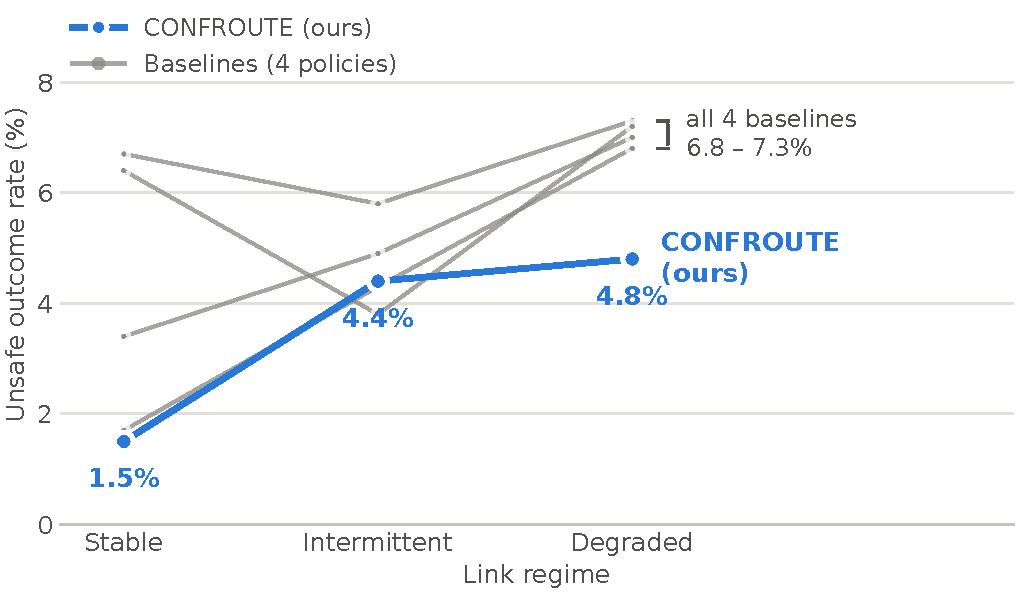
\includegraphics[width=\linewidth]{figures/fig_unsafe_by_scenario.pdf}
\end{column}
\begin{column}{0.35\textwidth}
  {\small On \textbf{stable} links, offloading is easy and everything that offloads does well.}
  \vspace{0.7em}

  {\small On \textbf{degraded} links, the four baselines converge on \num{6.8--7.3\%} because their escape hatch is gone.}
  \vspace{0.7em}

  {\small CONFROUTE holds at \num{4.8\%} by not attempting fragile offloads, and by refusing a bounded subset of tasks outright.}
\end{column}
\end{columns}
\end{frame}

% =============================================================================
% 13. Degraded trade-off
% =============================================================================
\begin{frame}{Result: under degraded links, safer \emph{and} faster}
\framesubtitle{Every policy under the degraded regime. Lower-left is better.}

\vspace{-0.2em}
\begin{columns}[c]
\begin{column}{0.62\textwidth}
  \centering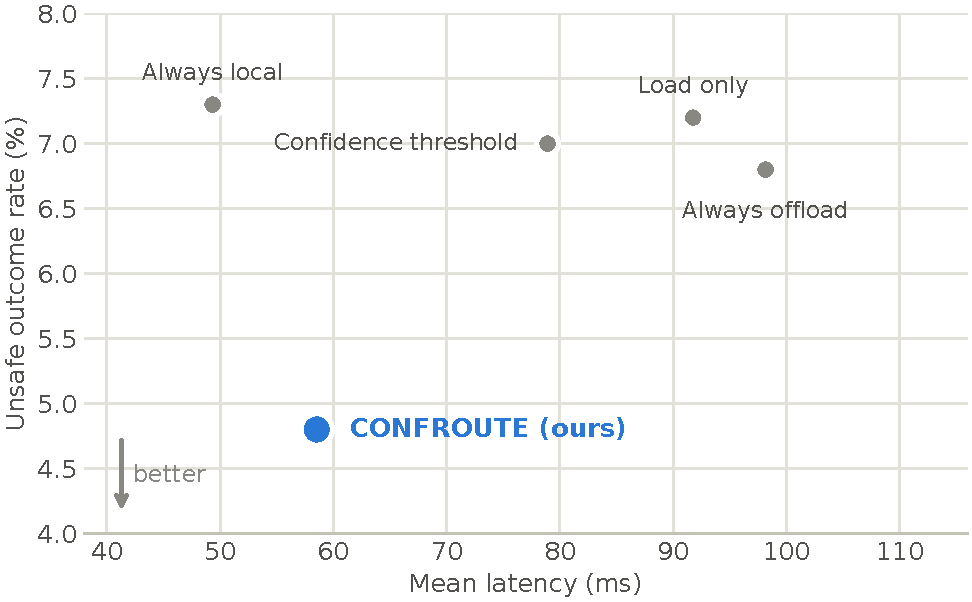
\includegraphics[width=\linewidth]{figures/fig_tradeoff.pdf}
\end{column}
\begin{column}{0.36\textwidth}
  \callout[wash]{\small vs. always-offload:\\[0.35em]
  unsafe \num{6.8\% $\rightarrow$ 4.8\%}\\[0.25em]
  latency \num{98.2 $\rightarrow$ 58.5\,ms}}
  \vspace{0.8em}

  {\small Always-local is the only faster policy, and it is the \emph{least} safe of all at 7.3\%.}
  \vspace{0.7em}

  {\color{ink2}\small Refusing to attempt an offload that will fail buys back both latency and safety at once.}
\end{column}
\end{columns}
\end{frame}

% =============================================================================
% 14. The honest table
% =============================================================================
\begin{frame}{Where we do \emph{not} win: intermittent links}
\framesubtitle{The regime in which offloading still mostly works}

\vspace{0.5em}
\centering
{\small
\begin{tabular}{@{}lrrrr@{}}
\toprule
\textbf{\color{navy}Policy} & \textbf{\color{navy}Latency (ms)} & \textbf{\color{navy}Unsafe} & \textbf{\color{navy}Energy (J)} & \textbf{\color{navy}Fallback} \\
\midrule
Always local          & \textbf{49.4} & 5.8\% & 0.50 & 0.0\% \\
Always offload        & 71.6 & 4.3\% & 0.59 & 0.0\% \\
Confidence threshold  & 59.6 & 4.9\% & \textbf{0.53} & 0.0\% \\
Load only             & 67.0 & \textbf{3.8\%} & 0.57 & 0.0\% \\
\hl{CONFROUTE (ours)} & \hl{61.6} & \hl{4.4\%} & \hl{0.56} & \hl{2.6\%} \\
\bottomrule
\end{tabular}}

\vspace{1.0em}
\begin{minipage}{0.88\textwidth}
\callout[washorange]{\small \textbf{Load-only routing is safer here} (3.8\% vs 4.4\%), at 5.4 ms more latency. When a peer is usually reachable, aggressive offloading is a reasonable strategy and our guardrails cost us a little. \shout{The case for CONFROUTE is the degraded regime}, which is also the regime that actually threatens the vessel.}
\end{minipage}
\end{frame}

% =============================================================================
% 15. Adaptation
% =============================================================================
\begin{frame}{The router shifts its behaviour with the link}
\framesubtitle{Action mix of CONFROUTE, 2,500 tasks per regime}

\vspace{0.1em}
\centering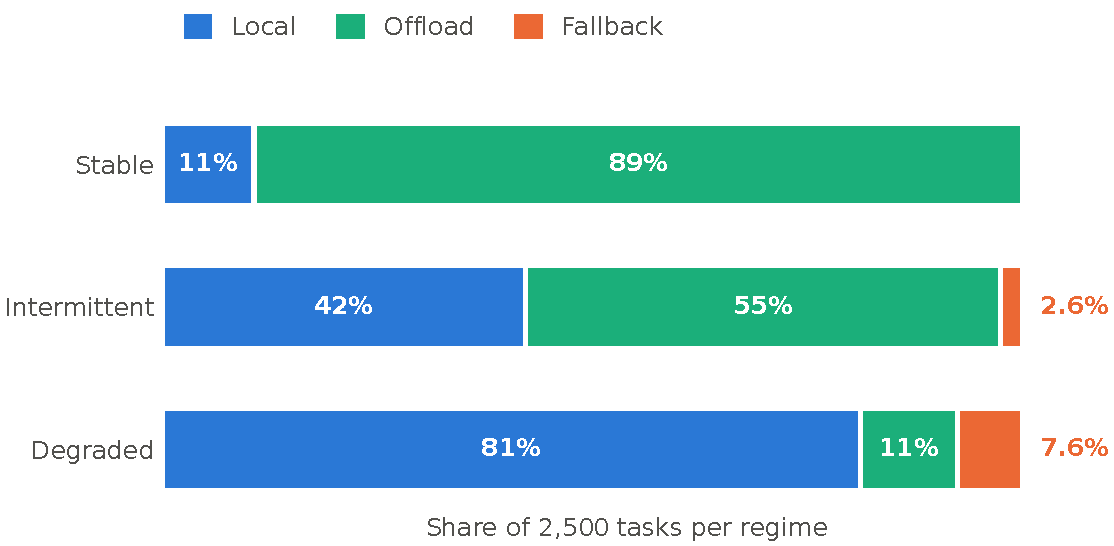
\includegraphics[width=0.76\textwidth]{figures/fig_actions.pdf}

\vspace{0.4em}
\begin{minipage}{0.86\textwidth}
{\small Offloading collapses from \num{89\%} to \num{11\%}, local execution absorbs most of it, and fallback rises to \num{7.6\%}. Fallback stays a \shout{bounded minority}: the vessel keeps operating.}
\end{minipage}
\end{frame}

% =============================================================================
% 16. Ablation
% =============================================================================
\begin{frame}{Ablation: both components are load-bearing}
\framesubtitle{Unsafe outcome rate under degraded links}

\vspace{1.2em}
\centering
{\large
\begin{tabular}{@{}lcc@{}}
\toprule
\textbf{\color{navy}Configuration} & \textbf{\color{navy}Unsafe rate} & \textbf{\color{navy}Significance} \\
\midrule
Full CONFROUTE               & \textbf{\color{cblue}4.8\%} & \\[0.35em]
Without the fallback action  & 6.2\% & $p = 0.012$ \\[0.35em]
Without link-state awareness & 5.9\% & $p = 0.037$ \\
\bottomrule
\end{tabular}}

\vspace{1.6em}
\begin{minipage}{0.82\textwidth}
{\small Removing fallback and forcing a local/offload binary costs more than removing link awareness. \shout{Having somewhere to put an undecidable task is the larger effect.}}
\end{minipage}
\end{frame}

% =============================================================================
% 17. The real bottleneck
% =============================================================================
\statement{The routing layer was never the bottleneck.}{%
We improved it, and unsafe outcomes still occur at high confidence.\\[0.6em]
Under distribution shift the classifier is \emph{more} certain and \emph{less} correct, so no policy reading max-softmax can be trusted to catch its own failures.}

% =============================================================================
% 18. What follows from that
% =============================================================================
\begin{frame}{What follows from that}

\vspace{0.5em}
\begin{columns}[T]
\begin{column}{0.48\textwidth}
  \textbf{\color{corange}Limitations we are explicit about}
  \begin{itemize}\setlength\itemsep{0.42em}\small
    \item Degradation is \emph{synthetic}, applied deterministically to satellite chips.
    \item One task family: image-chip classification. Not onboard perception, AIS trajectories or engine monitoring.
    \item Unsafe outcomes come from a routing-level cost model, not hardware-in-the-loop.
    \item Thresholds are fixed and trace-tuned.
  \end{itemize}
\end{column}
\begin{column}{0.48\textwidth}
  \textbf{\color{navy}Where we think the work goes}
  \begin{itemize}\setlength\itemsep{0.42em}\small
    \item \shout{Calibration first}: temperature scaling, conformal prediction, explicit OOD and shift detection feeding the router.
    \item Adaptive thresholds via bandit feedback or Bayesian optimisation.
    \item Peer-aware forwarding: model version, accelerator, current load, discovered in ad-hoc maritime networks.
    \item Real link traces and hardware-in-the-loop validation.
  \end{itemize}
\end{column}
\end{columns}

\vspace{0.7em}
{\color{ink2}\small Fallback rate and unsafe-local rate have different operational meanings, so we recommend both always be reported separately. A policy can look safe by refusing everything.}
\end{frame}

% =============================================================================
% 19. Takeaways
% =============================================================================
\begin{frame}{Three things to take away}

\vspace{1.0em}
\begin{enumerate}\setlength\itemsep{1.1em}
  \item[\textbf{\color{cblue}1}] \textbf{Fallback deserves to be a routing action.} Under degraded links it cuts unsafe outcomes from 6.8\% to 4.8\% and saves 40 ms, because a failed offload costs both.
  \item[\textbf{\color{cblue}2}] \textbf{Confidence thresholds break exactly when needed.} Under maritime degradation, accuracy falls 13.8 points while confidence rises, and 90\% of errors clear the threshold.
  \item[\textbf{\color{cblue}3}] \textbf{Calibration is the reliability bottleneck for maritime edge AI}, ahead of routing or scheduling optimisation. Safe autonomy at sea depends on knowing what the model does not know.
\end{enumerate}

\vspace{1.4em}
{\color{rule}\hrule height 0.7pt}
\vspace{0.7em}
\begin{columns}[T]
\begin{column}{0.55\textwidth}
{\color{navy}\large\bfseries Thank you. Questions?}
\end{column}
\begin{column}{0.43\textwidth}
{\color{ink2}\footnotesize Anthony Uchenna Eneh\\ anthony@kumoh.ac.kr\\ Kumoh National Institute of Technology}
\end{column}
\end{columns}
\end{frame}

% =============================================================================
% Backup
% =============================================================================
{\setbeamertemplate{footline}{}
\begin{frame}[plain]
  \vfill\centering{\color{muted}\Large Backup}\vfill
\end{frame}}

\begin{frame}{Backup: full results, all policies and regimes}

\vspace{0.4em}
\centering
{\footnotesize
\begin{tabular}{@{}llrrr@{}}
\toprule
\textbf{\color{navy}Policy} & \textbf{\color{navy}Regime} & \textbf{\color{navy}Latency (ms)} & \textbf{\color{navy}Unsafe} & \textbf{\color{navy}Energy (J)} \\
\midrule
Always local        & Stable       & 49.3 & 6.7\% & 0.50 \\
Always offload      & Stable       & 33.4 & 1.7\% & 0.60 \\
Confidence threshold& Stable       & 46.5 & 3.4\% & 0.53 \\
Load only           & Stable       & 48.2 & 6.4\% & 0.51 \\
\hl{CONFROUTE} & \hl{Stable} & \hl{33.5} & \hl{1.5\%} & \hl{0.60} \\
\midrule
Always local        & Intermittent & 49.4 & 5.8\% & 0.50 \\
Always offload      & Intermittent & 71.6 & 4.3\% & 0.59 \\
Confidence threshold& Intermittent & 59.6 & 4.9\% & 0.53 \\
Load only           & Intermittent & 67.0 & 3.8\% & 0.58 \\
\hl{CONFROUTE} & \hl{Intermittent} & \hl{61.6} & \hl{4.4\%} & \hl{0.56} \\
\midrule
Always local        & Degraded     & 49.3 & 7.3\% & 0.50 \\
Always offload      & Degraded     & 98.2 & 6.8\% & 0.56 \\
Confidence threshold& Degraded     & 78.9 & 7.0\% & 0.55 \\
Load only           & Degraded     & 91.8 & 7.2\% & 0.56 \\
\hl{CONFROUTE} & \hl{Degraded} & \hl{58.5} & \hl{4.8\%} & \hl{0.50} \\
\bottomrule
\end{tabular}}
\end{frame}

\begin{frame}{Backup: the routing cost model}

\vspace{1.2em}
\begin{equation*}
  C(r_i) = w_1 \cdot \ell(r_i) \;+\; w_2 \cdot e(r_i) \;+\; w_3 \cdot \mathbf{1}_{\text{unsafe}}(r_i) \cdot \Delta_{\text{safety}}
\end{equation*}

\vspace{1.2em}
\begin{itemize}\setlength\itemsep{0.55em}
  \item $\ell(r_i)$ latency, $e(r_i)$ energy under the chosen action.
  \item $\mathbf{1}_{\text{unsafe}}(r_i)$ marks a wrong high-impact decision; $\Delta_{\text{safety}}$ is the safety penalty.
  \item The policy minimises expected cost under uncertainty about connectivity, resource state and model confidence.
  \item \shout{Fallback is optimal} whenever it avoids a large $\Delta_{\text{safety}}$ under low confidence and a poor link.
\end{itemize}

\vspace{1.0em}
{\color{ink2}\small Task $x_i = (d_i, g_i, s_i)$: sensor payload, urgency class, platform state. Action $r_i \in \{\text{local}, \text{forward}, \text{fallback}\}$.}
\end{frame}

\begin{frame}{Backup: confidence traces}

\vspace{1.2em}
\centering
{\large
\begin{tabular}{@{}lrrrr@{}}
\toprule
\textbf{\color{navy}Condition} & \textbf{\color{navy}Samples} & \textbf{\color{navy}Accuracy} & \textbf{\color{navy}Mean conf.} & \textbf{\color{navy}Std.} \\
\midrule
Nominal & 500 & 88.8\% & 0.810 & 0.140 \\
Adverse & 500 & 75.0\% & 0.842 & 0.085 \\
\bottomrule
\end{tabular}}

\vspace{1.6em}
\begin{minipage}{0.86\textwidth}
{\small The adverse transform is deterministic: reduced contrast and brightness, Gaussian blur, haze blending, and sensor-like noise. Note the \emph{narrowing} standard deviation: the model is not just wrong, it is uniformly confident.}

\vspace{0.9em}
{\small Mean confidence on incorrect predictions: \num{0.651} nominal, \num{0.782} adverse.\\
Errors above the 0.65 fallback threshold: \num{22 of 56} nominal, \num{113 of 125} adverse.}
\end{minipage}
\end{frame}

\end{document}
